\chapter{Analysis}
\label{Analysis_chapter}

Since MadGraph needs as input parameter the mass of the heavy neutrino, two signals were simulated with different values of mass. One signal was simulated with a neutrino mass of 5.0 GeV, while the other one used a value of 70.0 GeV.

In order to study the performance of a variable to reduce the background, histograms of this variable were made for each signal and background. The type of histograms used in this analysis are called stacked plots. In these histograms each distribution of the variable is placed on the same plot and each one is normalized to the cross section and luminosity. The luminosity expected for the LHC accelerator by the end of 2017 is 50 $fb^{-1}$. This normalization makes possible to compare the behavior of a given variable for the signal with respect to the given background. In stacked plots the backgrounds are placed sequentially on top of each other, in order to represent a graphical sum of the total noise contribution in the analysis. The signal is drawn overlaid on top of the background. The statistical uncertainty is represented by a dashed line at the top of the background histograms. The plots shown here include just the W+jets and DY+jets backgrounds, because these are very large compared to the $t\overline{t}$ background, and reducing them is already a difficult task.

In the first four plots showed in this chapter some cuts were imposed: the preselection cuts and cuts on the number of jets, taus and b-jets. Figure \ref{MET_bjets} shows the stacked plot of $\vec{E_T^{miss}}$. It can be seen that the quantity of background events is much larger than the number of events of both signals at any value of $\vec{E_T^{miss}}$. Moreover, the distribution shape of both backgrounds is alike to the shape of both signals. This implies that a cut on this variable would reduce the background in a similar way as it would reduce the signal. Thus, it is not possible to find an optimal $\vec{E_T^{miss}}$ cut value.

 \begin{figure}[h] 
 \centering
 \caption{Stacked plot of $E_T^{miss}$ after the preselection cuts and cuts on the number of jets, taus and b-jets.}
 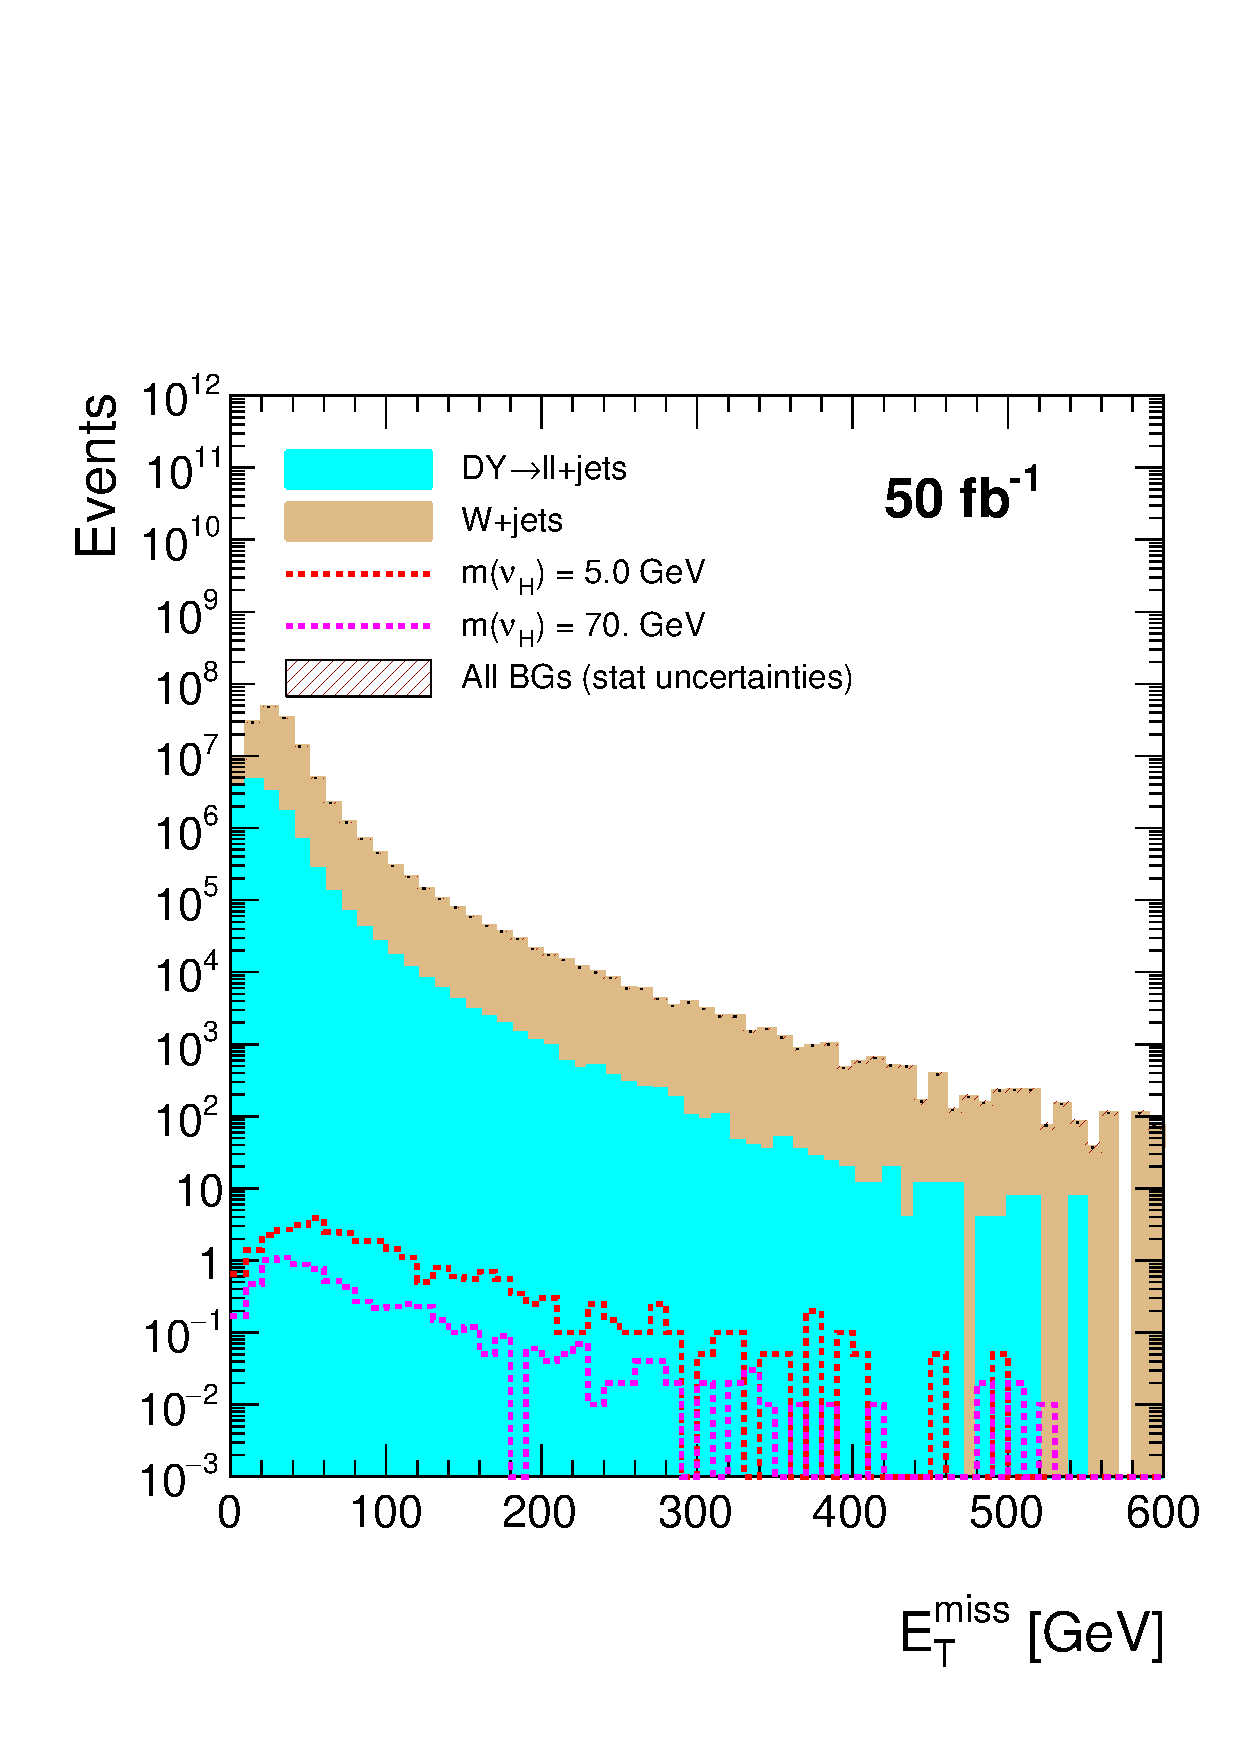
\includegraphics[width=0.8\textwidth]{./Capitulos/Analysis/AfterBJets/MET_MET_20} 
 \label{MET_bjets}
 \end{figure}
 
We studied the distribution of more variables in order to find possible cut values that can reduce the contribution of background. Figures \ref{HT_bjets}, \ref{diJetMass_bjets} and \ref{taupt_bjets} show the stacked plots of the variables $H_T$, di-jet mass and the tau $p_T$, respectively. These plots follow an analogous behavior as in the case of $\vec{E_T^{miss}}$: the number of background events is larger than of signal events and the background distribution is similar to the signal distribution. As a consequence, it is not possible to determine a set of variables that allow to reduce the contribution of background.
 
 \begin{figure}[h] 
 \centering
 \caption{Stacked plot of $H_T$ after the preselection cuts and cuts on the number of jets, taus and b-jets.}
 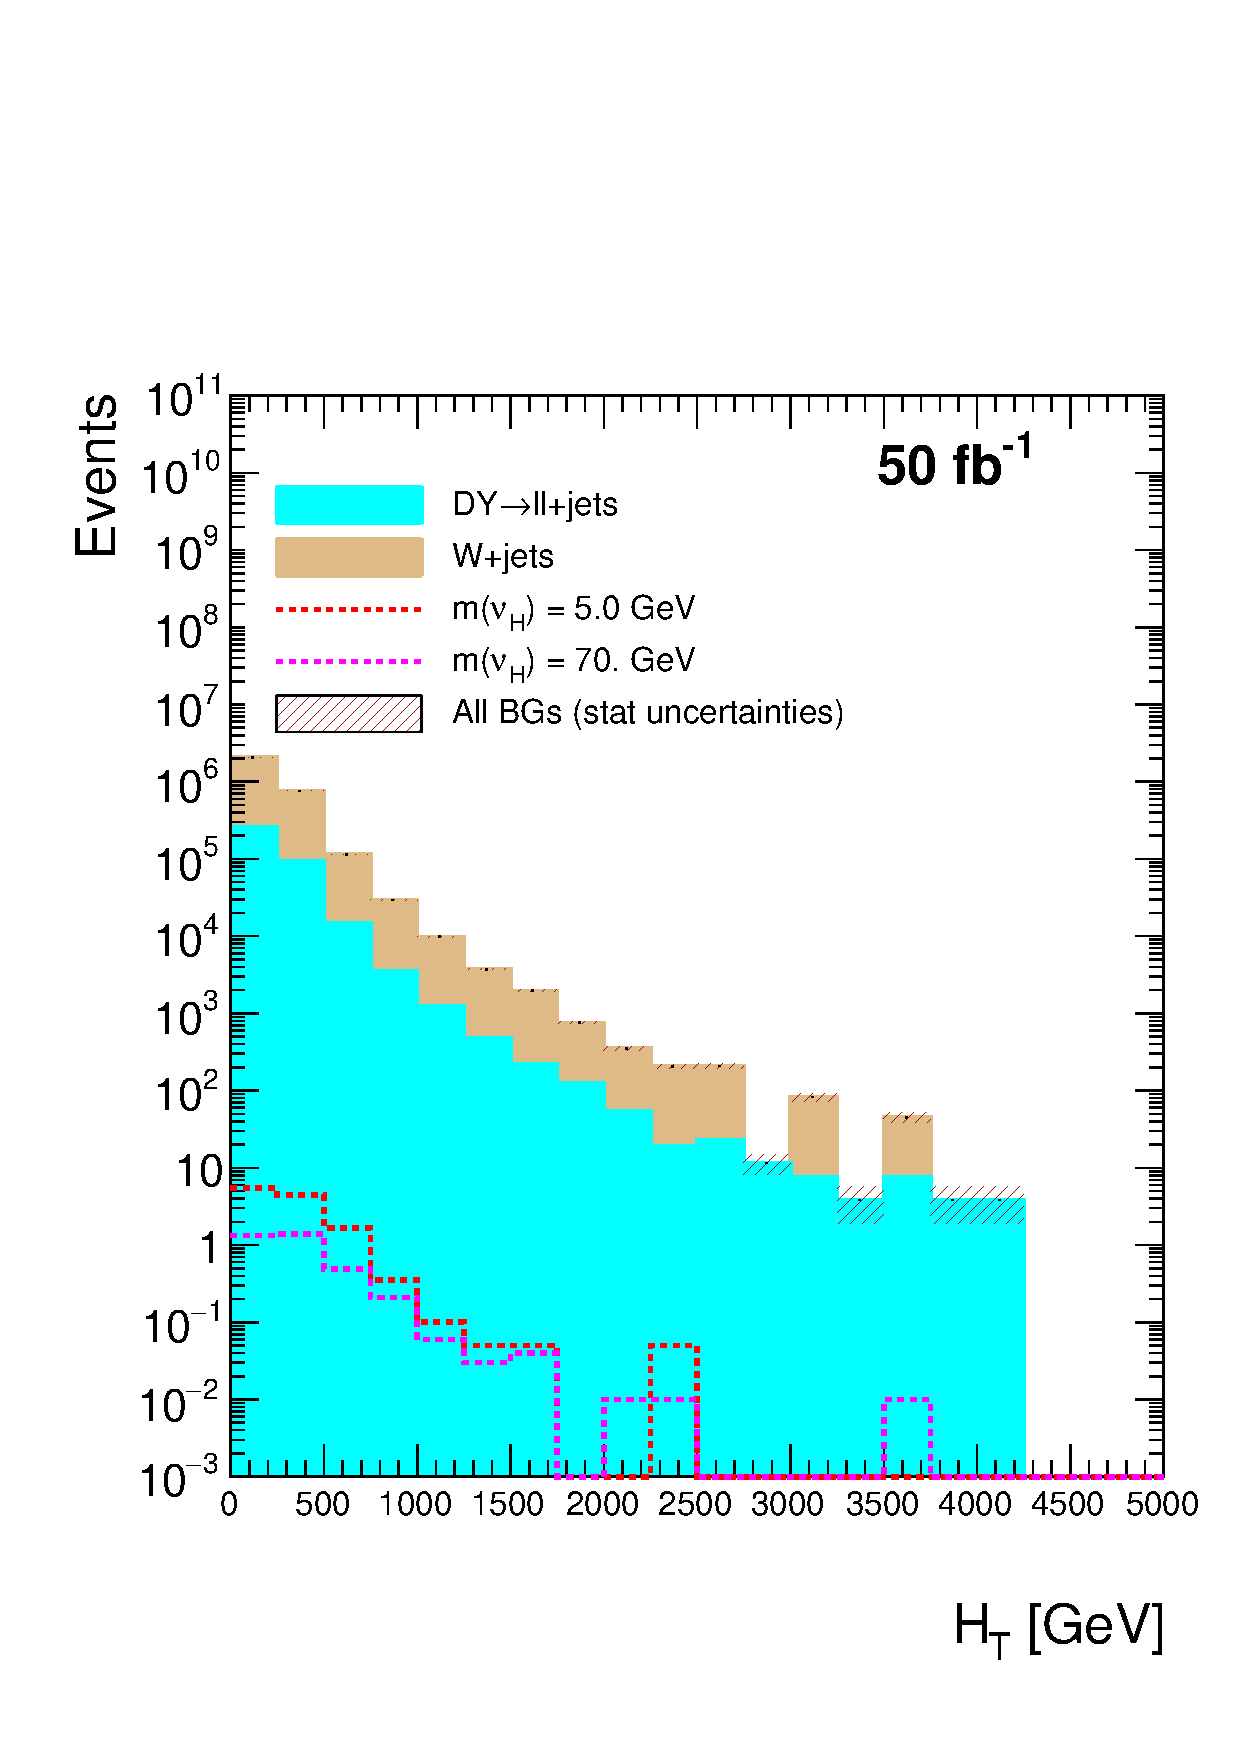
\includegraphics[width=0.7\textwidth]{./Capitulos/Analysis/AfterBJets/HT_MET_20} 
 \label{HT_bjets}
 \end{figure} 
 
  \begin{figure}[h] 
 \centering
 \caption{Stacked plot of di-jet mass after the preselection cuts and cuts on the number of jets, taus and b-jets.}
 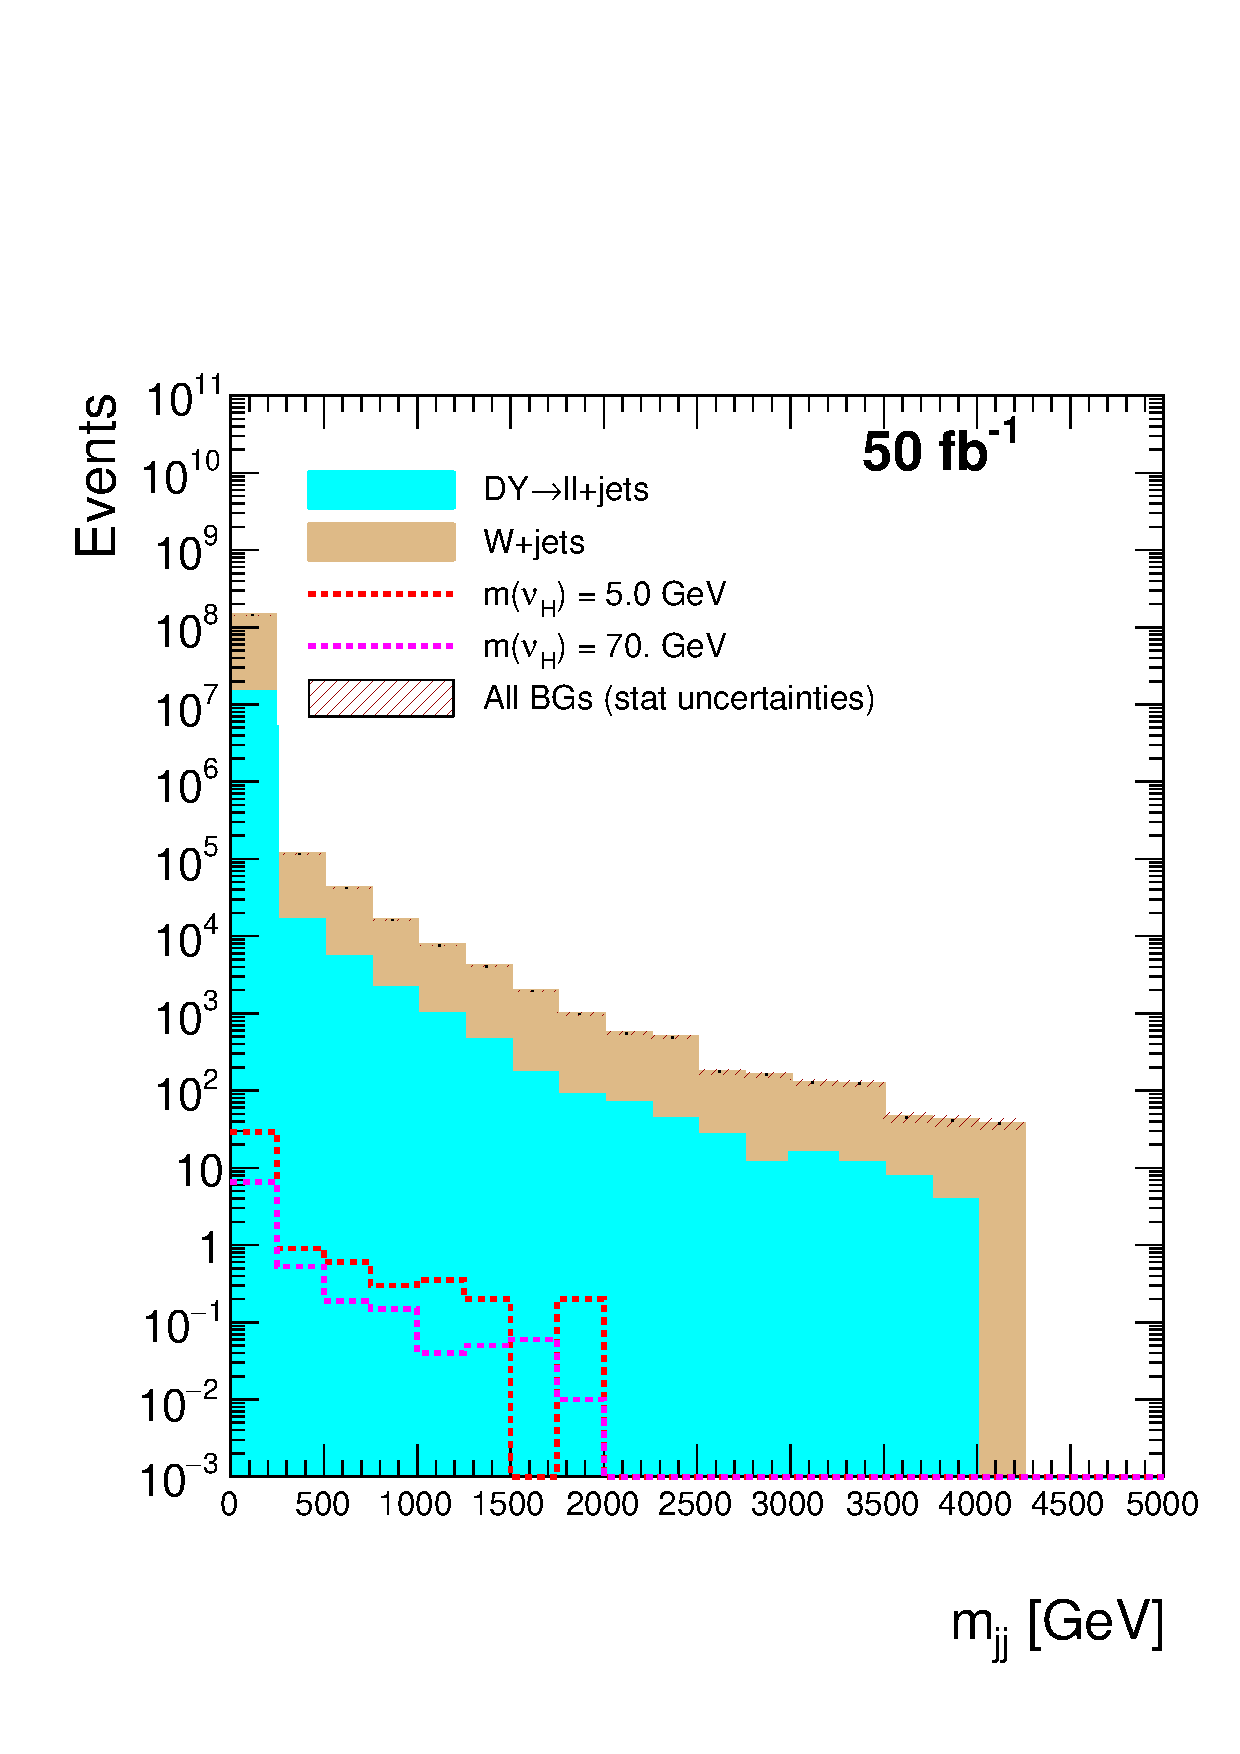
\includegraphics[width=0.7\textwidth]{./Capitulos/Analysis/AfterBJets/mjj_MET_20} 
 \label{diJetMass_bjets}
 \end{figure} 
 
  \begin{figure}[h] 
 \centering
 \caption{Stacked plot of $p_T(\tau)$ after the preselection cuts and cuts on the number of jets, taus and b-jets.}
 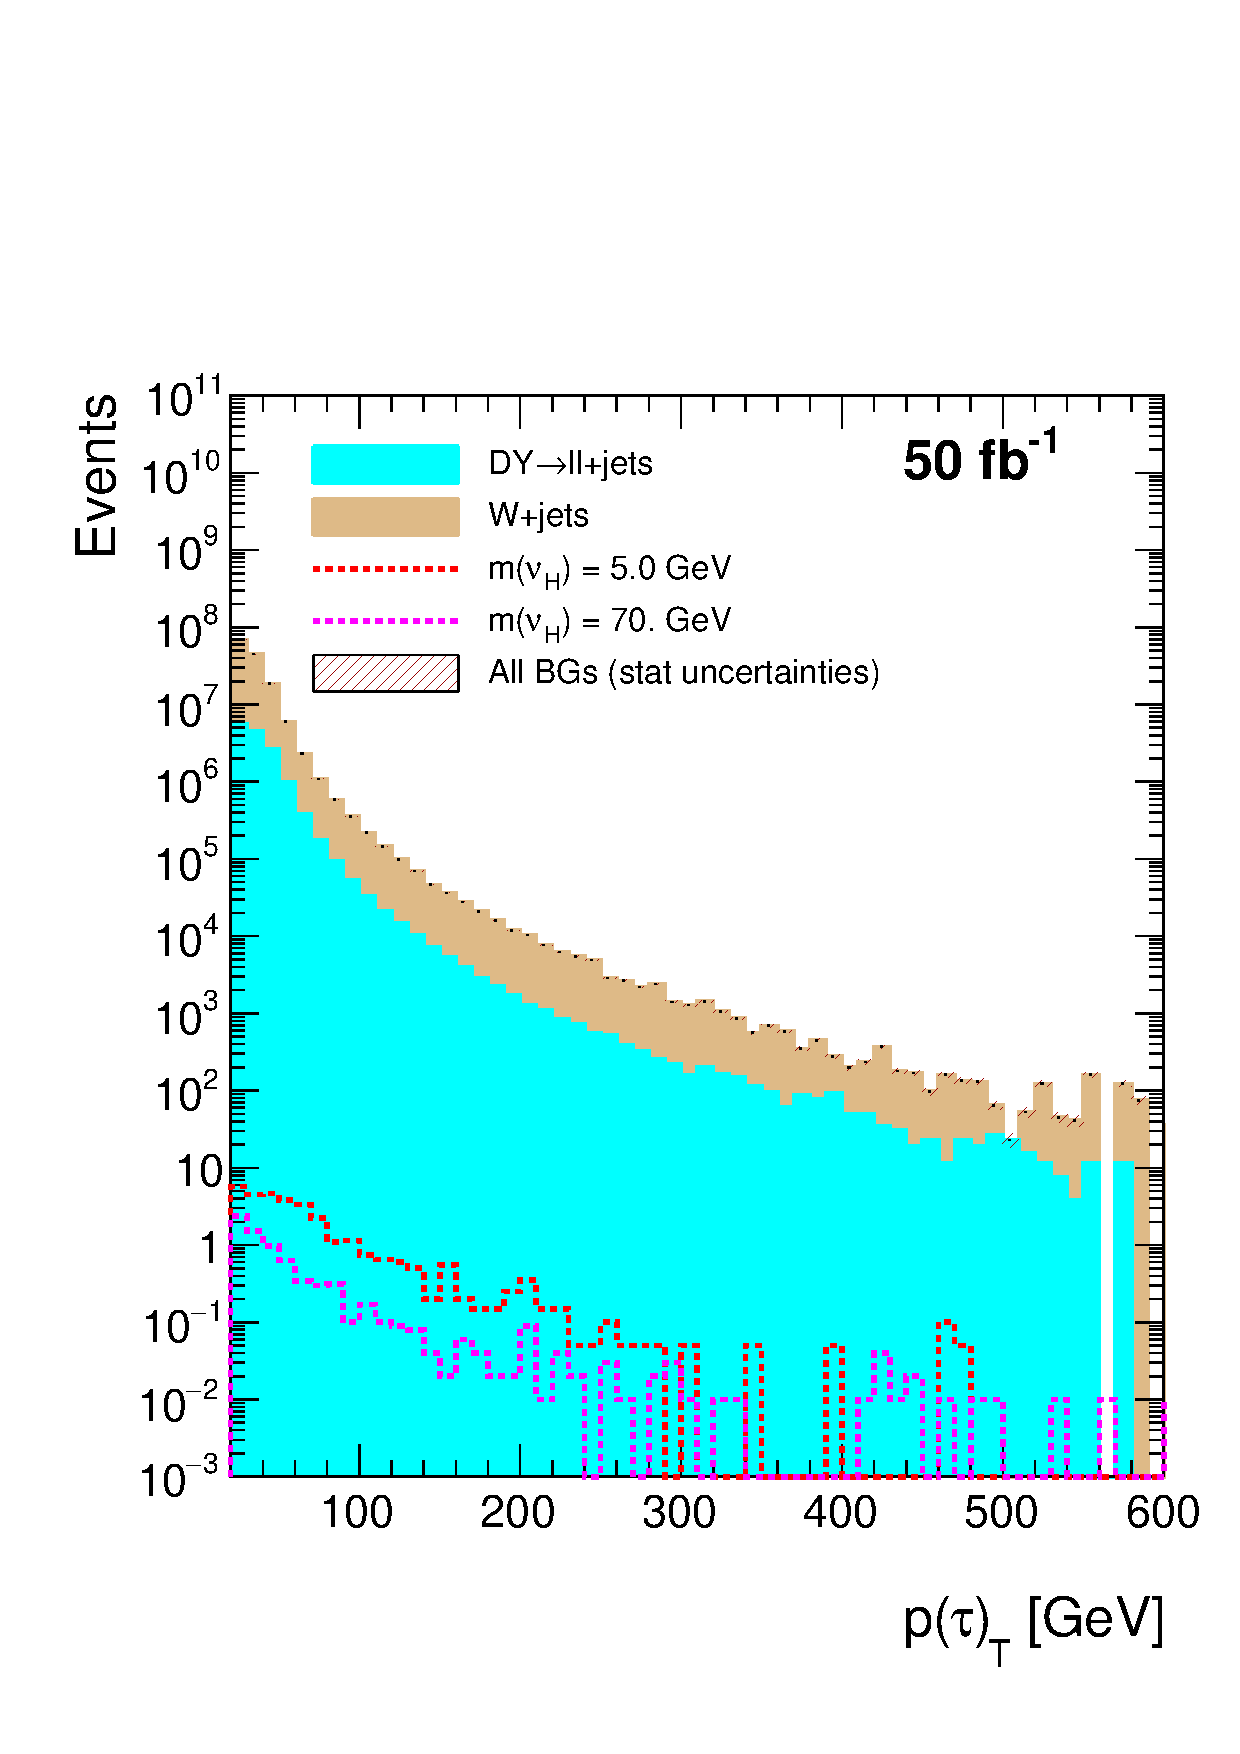
\includegraphics[width=0.7\textwidth]{./Capitulos/Analysis/AfterBJets/TauPt_MET_20} 
 \label{taupt_bjets}
 \end{figure} 
 
 Then, all the cuts mentioned in the Chapter \ref{Event_selection_criteria_chapter} are imposed. 
 These cuts include the cuts which take into account the topology of VBF processes. Figures \ref{HT_VBF}, \ref{diJetMass_VBF} and \ref{taupt_VBF} show the stacked plots of the $H_T$, di-jet mass and tau $p_T$ variables after all cuts, respectively. It can be seen that the quantity of background events reduces drastically, but it is still larger than the number of signal events. Moreover, the amount of signal events after imposing all cuts is minimal. Thus, it was not achievable to find a set of cuts that could reduce the background contribution in order to distinguish our signal of interest.
  
 
 \begin{figure}[h] 
 \centering
 \caption{Stacked plot of $H_T$ after the all the cuts were imposed.}
 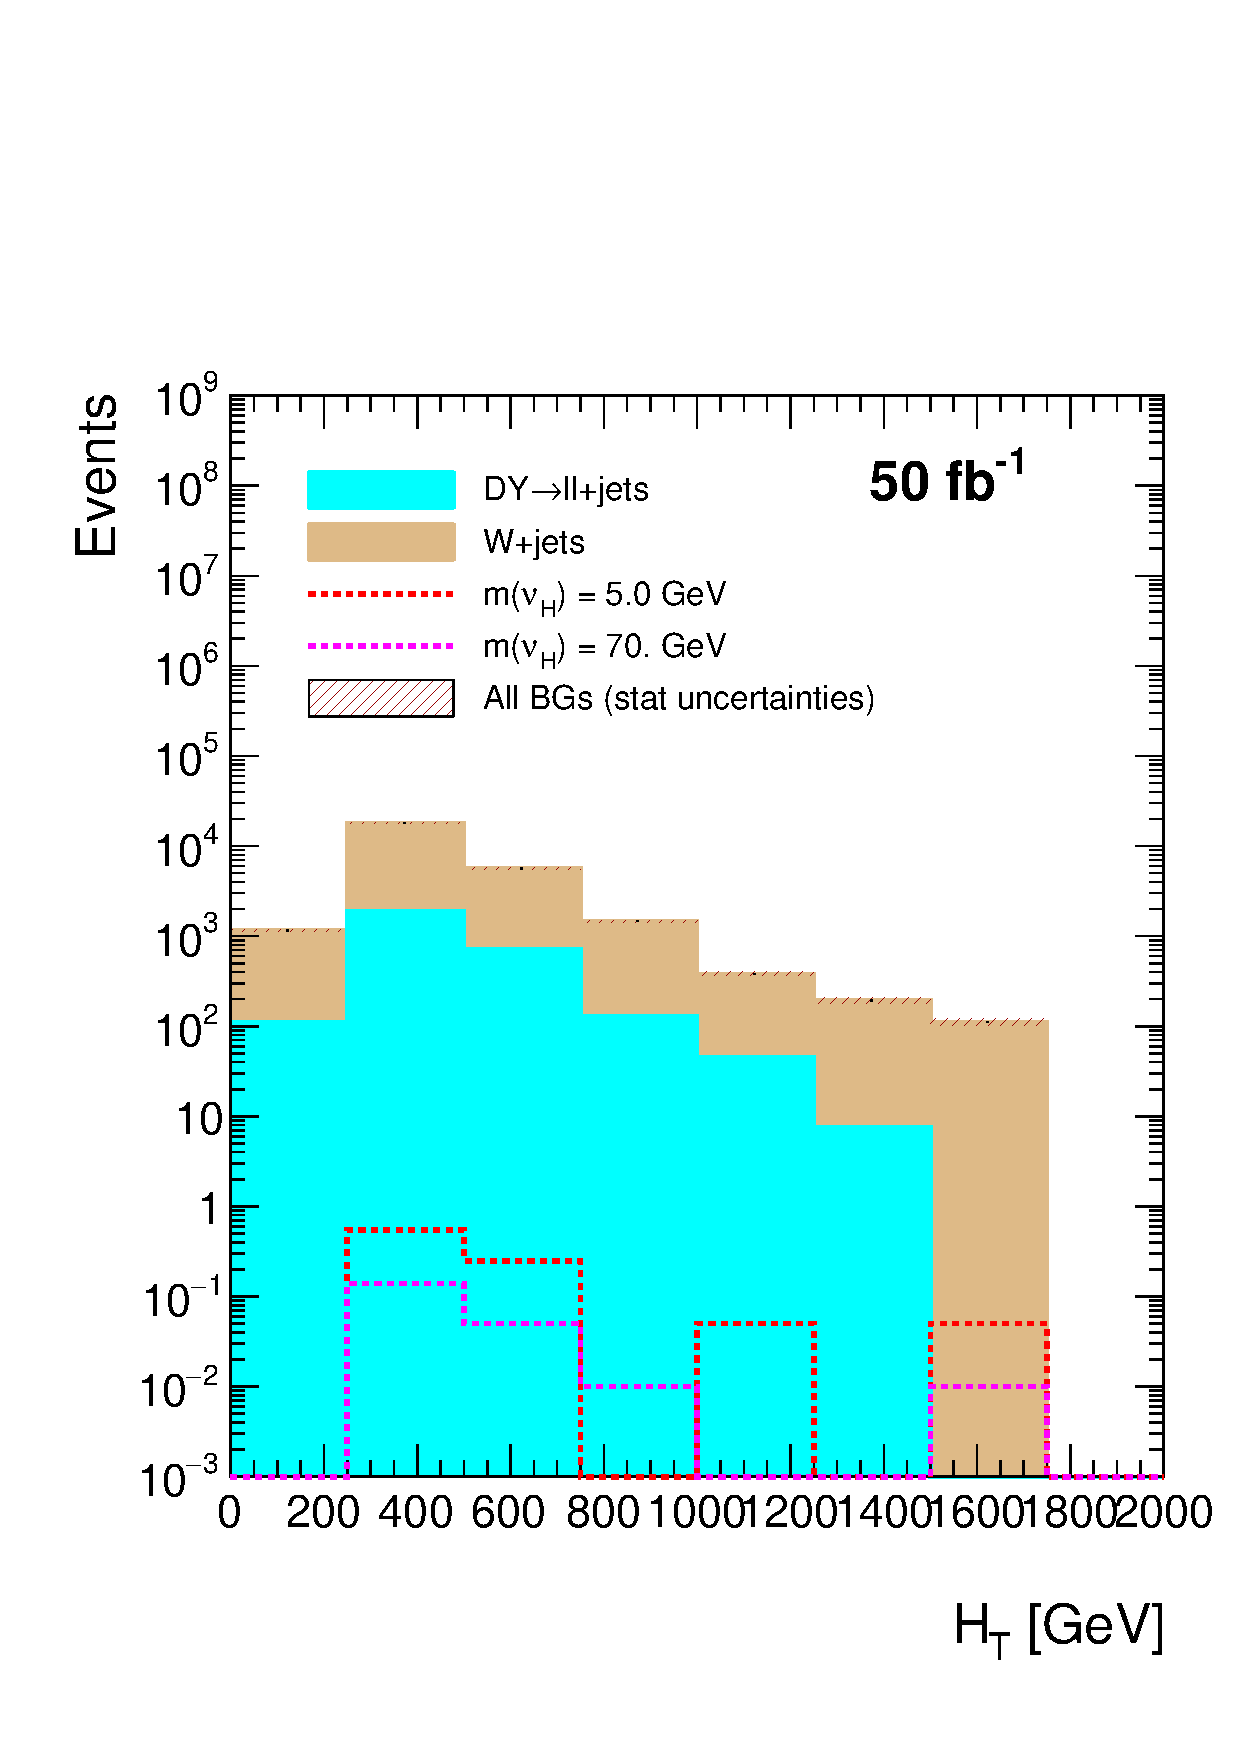
\includegraphics[width=0.7\textwidth]{./Capitulos/Analysis/AfterVBFCUTS/HT_MET_20} 
 \label{HT_VBF}
 \end{figure} 
 
  \begin{figure}[h] 
 \centering
 \caption{Stacked plot of di-jet mass after the all the cuts were imposed.}
 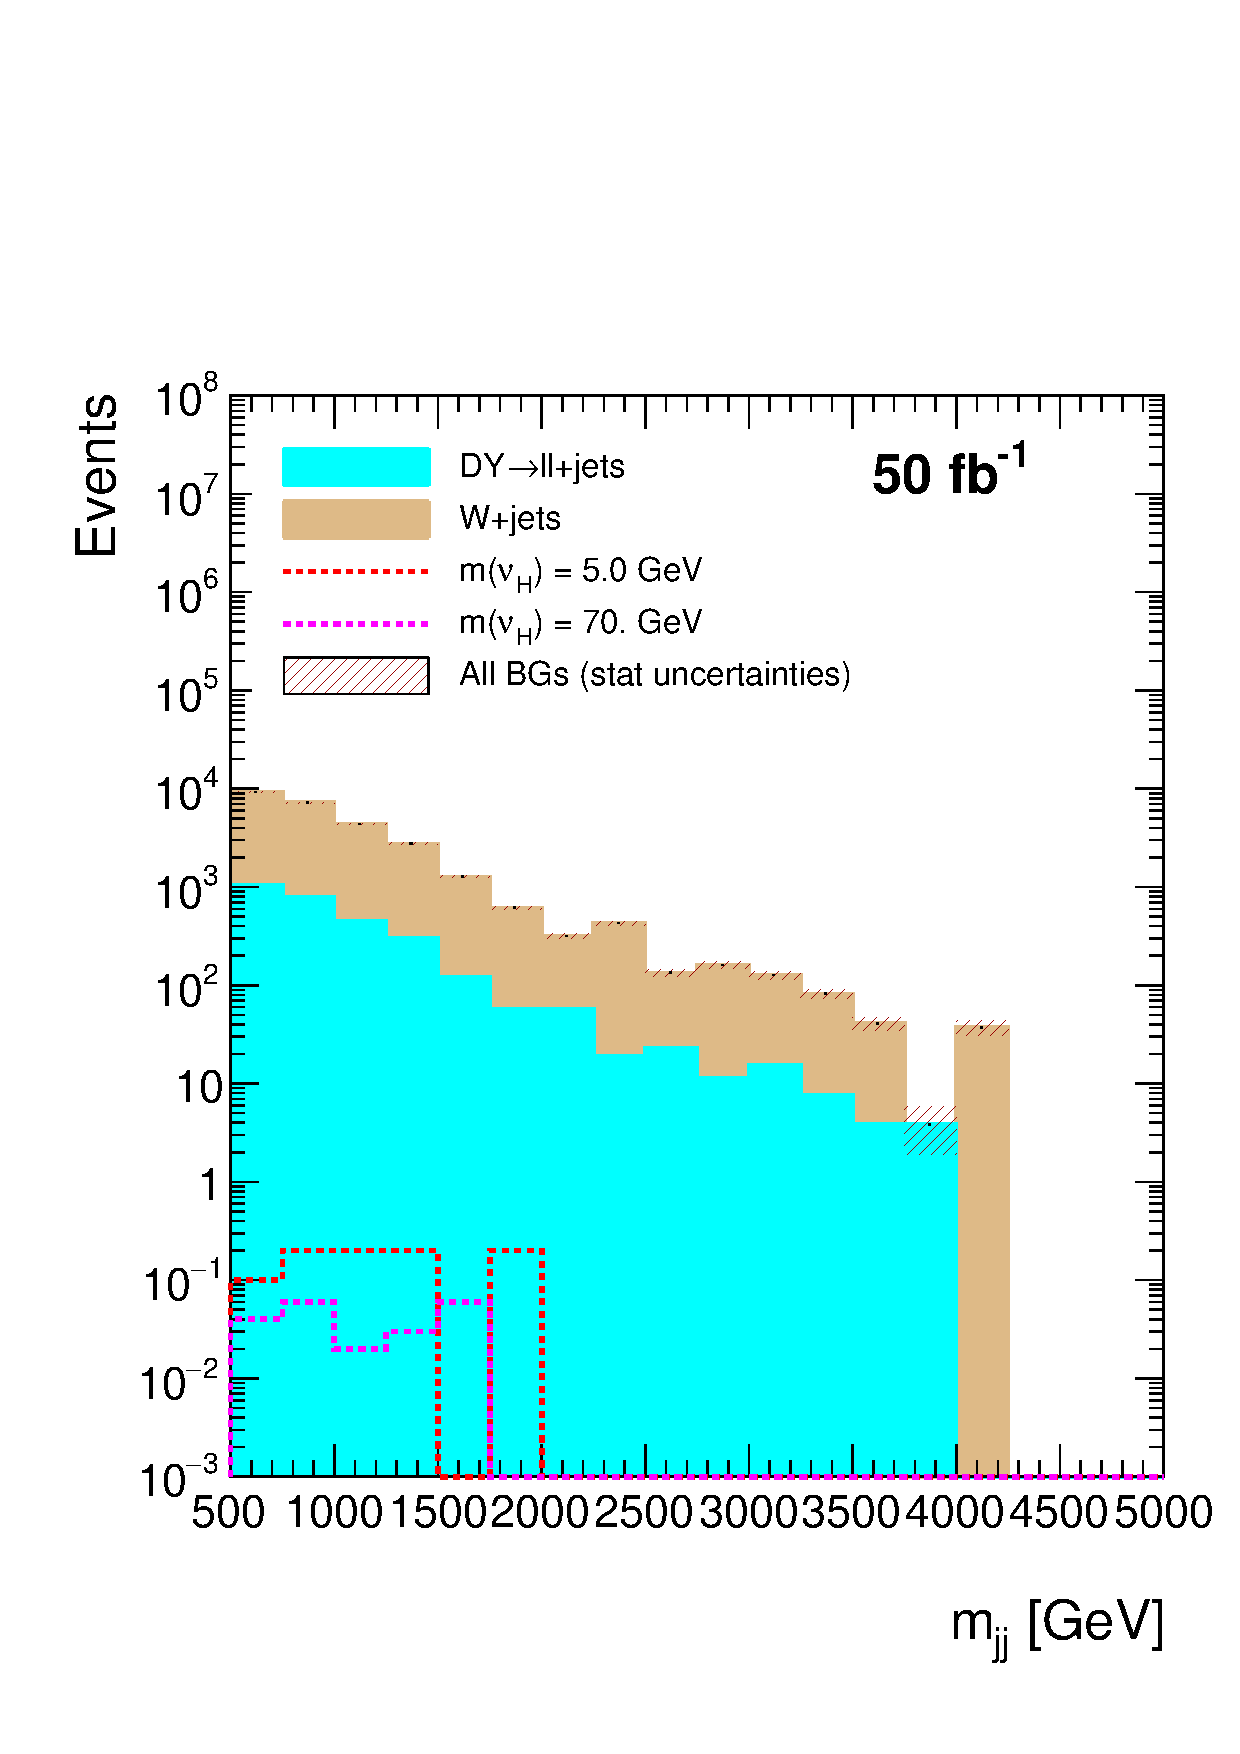
\includegraphics[width=0.7\textwidth]{./Capitulos/Analysis/AfterVBFCUTS/mjj_MET_20} 
 \label{diJetMass_VBF}
 \end{figure} 
 
  \begin{figure}[h] 
 \centering
 \caption{Stacked plot of $p_T(\tau)$ after the all the cuts were imposed.}
 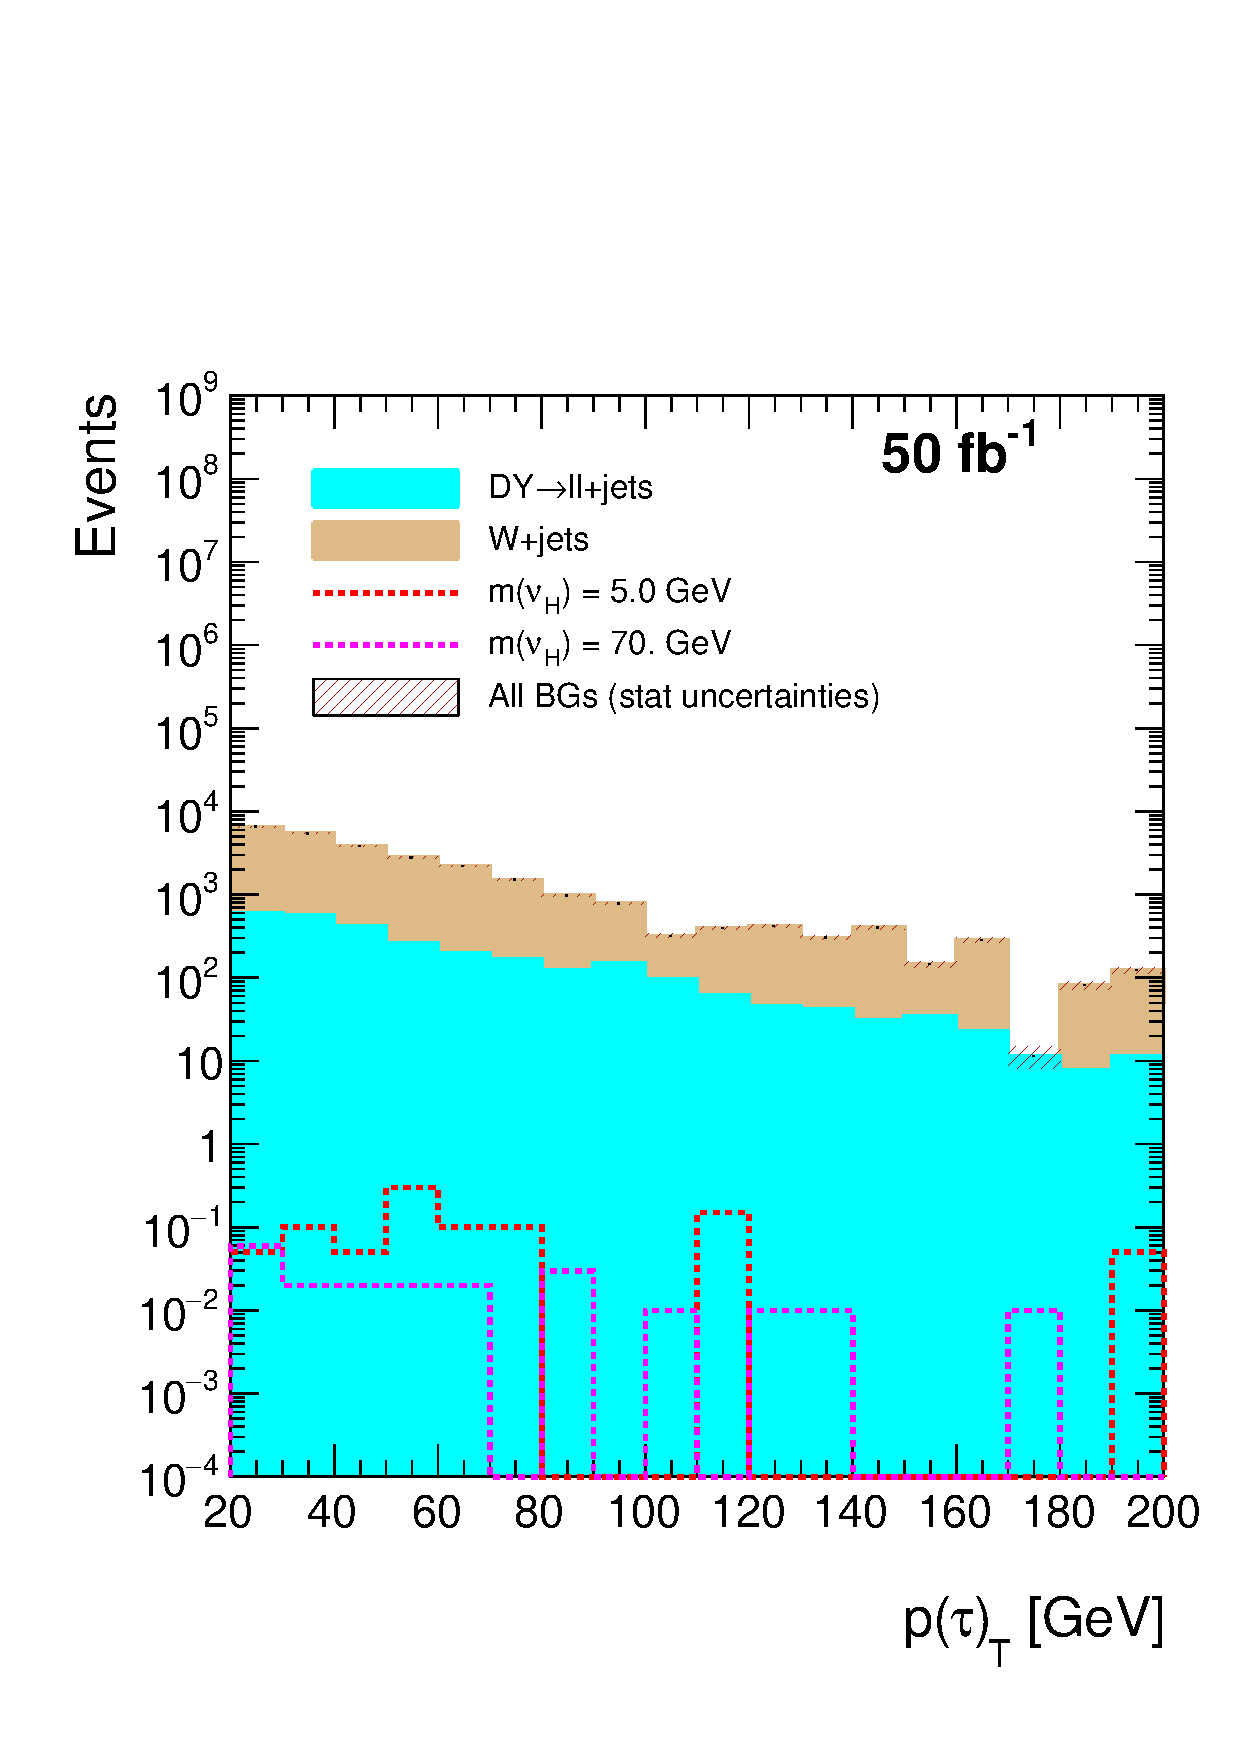
\includegraphics[width=0.7\textwidth]{./Capitulos/Analysis/AfterVBFCUTS/TauPt_MET20} 
 \label{taupt_VBF}
 \end{figure}  

One fact that can explain the reason why VBF cuts do not allow to reduce significantly the number of background events compared to the signal, is that the mass values of the Higgs boson and the Z boson are similar. Since this mass difference is almost just 30 GeV, the production mechanism of a Higgs boson is identical to the Z gamma production mechanism. Thus, the characteristics of the VBF jets in both events are similar and it is difficult to distinguish both VBF topologies. In the case that the heavy neutrinos are produced by the decay of a particle heavier that the Higgs boson, the heavier particle must be the result of an interaction between VBF jets with larger energy. Thus, in this case it would be expected that the detected VBF jets would be more energetic, which could allow to distinguish between both final states.

Since it was expected that the resulting tau in the signal had an associated track with a displaced vertex, some 2D plots were made using this variable. The value of the impact parameter for the tau was found by performing a minimization process on the distance between the tau and the tracks. 

First, we studied a plot on which the x axis 
represents $\vec{E_T^{miss}}$ and the y axis is the impact parameter ($d_{xy}$). This plot is shown in Figure \ref{ipt1_MET}. The first two plots at the left of this figure correspond to the signal events, one assuming a mass of the heavy neutrino of 5.0 GeV, and the other of 70.0 GeV. The range of the y axis for these plots is just from -1.0 to 1.0. The other two plots at the right of the figure correspond to the W+jets background and DY+jets background. These plots have a range in the y axis from -8.0 to 8.0. It can be seen that the impact parameter value of the signals is almost zero. This implies that it is not possible to make a cut on this variable to reduce the background as it was expected. Additionally, it is important to notice that in the case of the signals, the impact parameter only takes positive values which is not expected since the topology of the events should be symmetrical. 
 
 \begin{figure}[h] 
 \centering
 \caption{2D plot: $E_T^{miss}$ vs $d_{xy}$}
 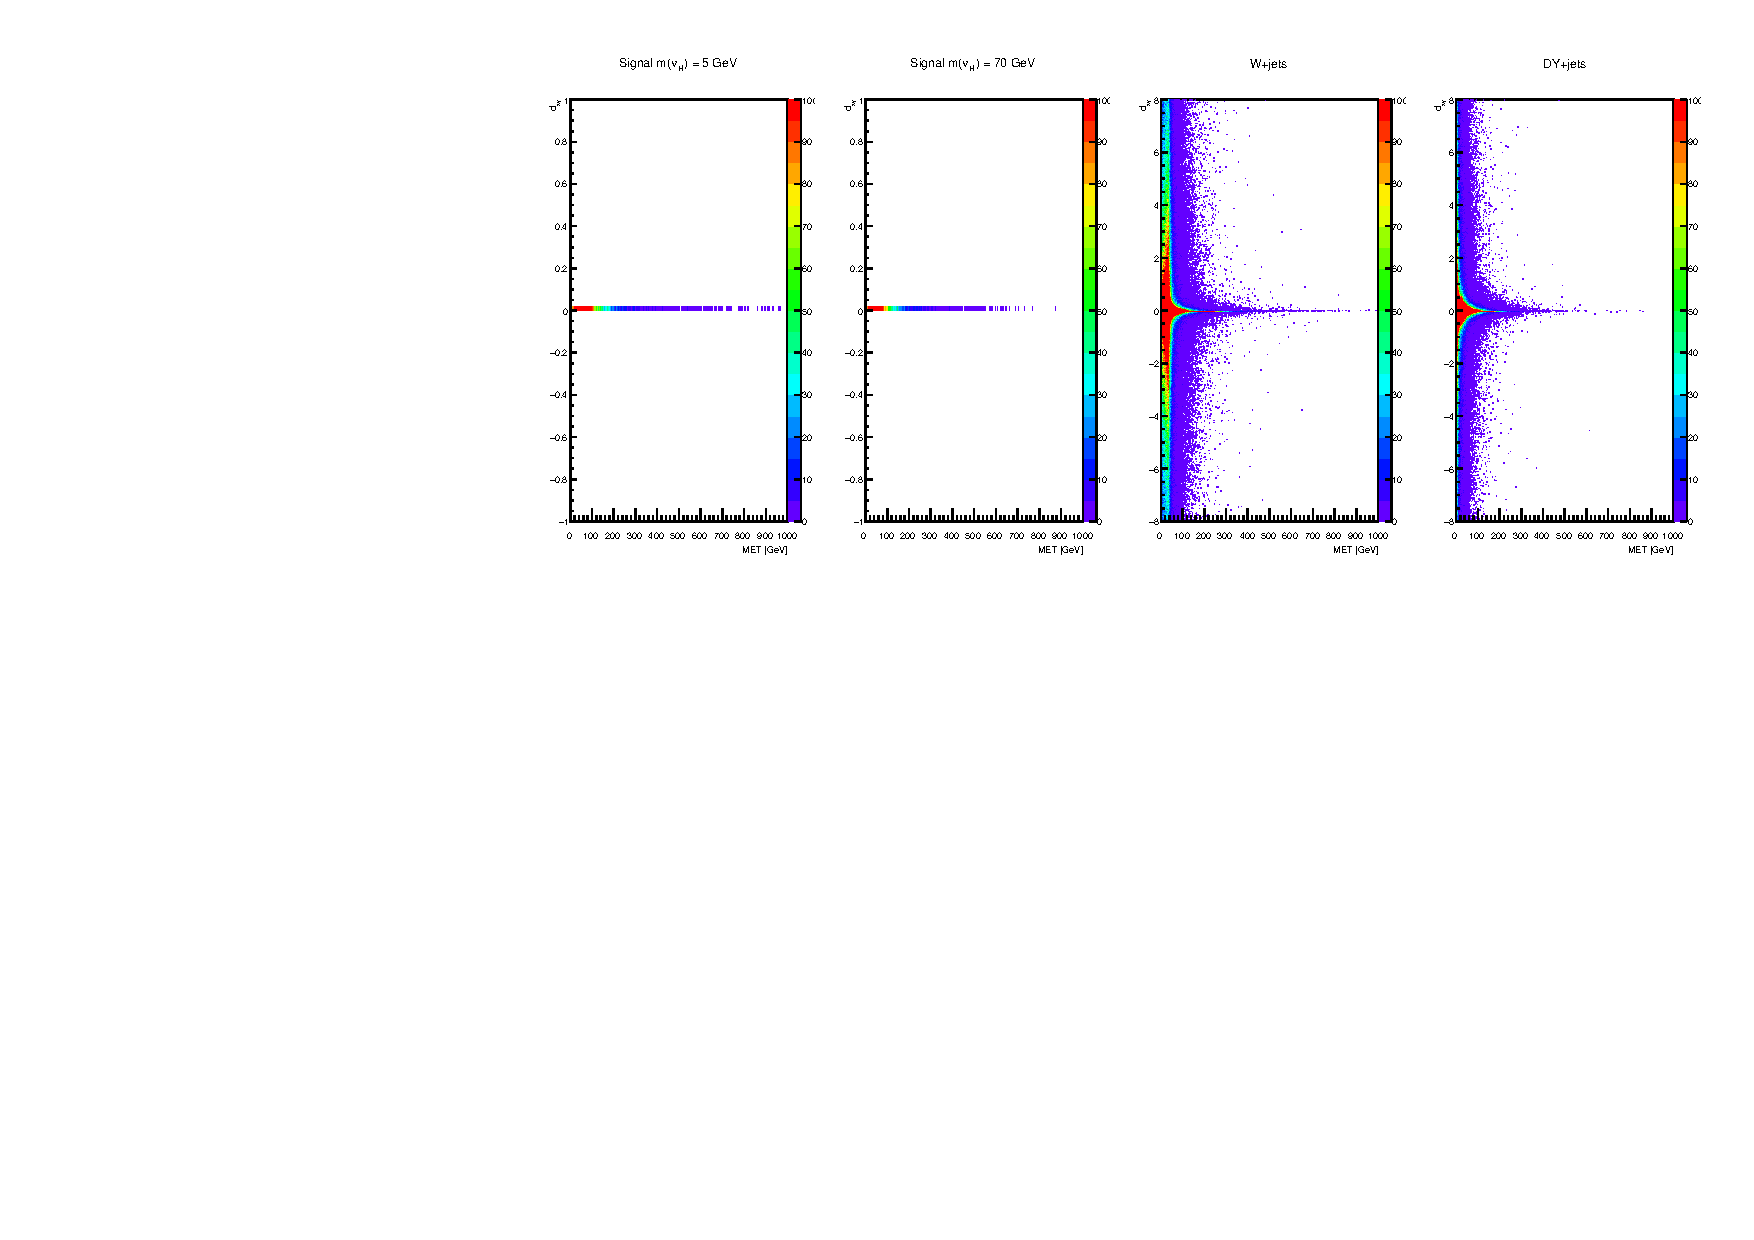
\includegraphics[width=1.15\textwidth]{./Capitulos/Analysis/c1} 
 \label{ipt1_MET}
 \end{figure}
 
Other 2D plots studied are shown in Figure \ref{ipt1_pt}. In these plots the x axis represents the tau transverse momentum and the y axis represents the absolute value of the impact parameter. In the signal plots, the y axis has a range between -0.1 to 0.4; while in the background plots it has a range between 0 and 8. Unfortunately, it is not possible to determine a cut value on any of these variables.
 
 \begin{figure}[h] 
 \centering
 \caption{2D plot: $p_T(\tau)$ vs $|d_{xy}|$}
 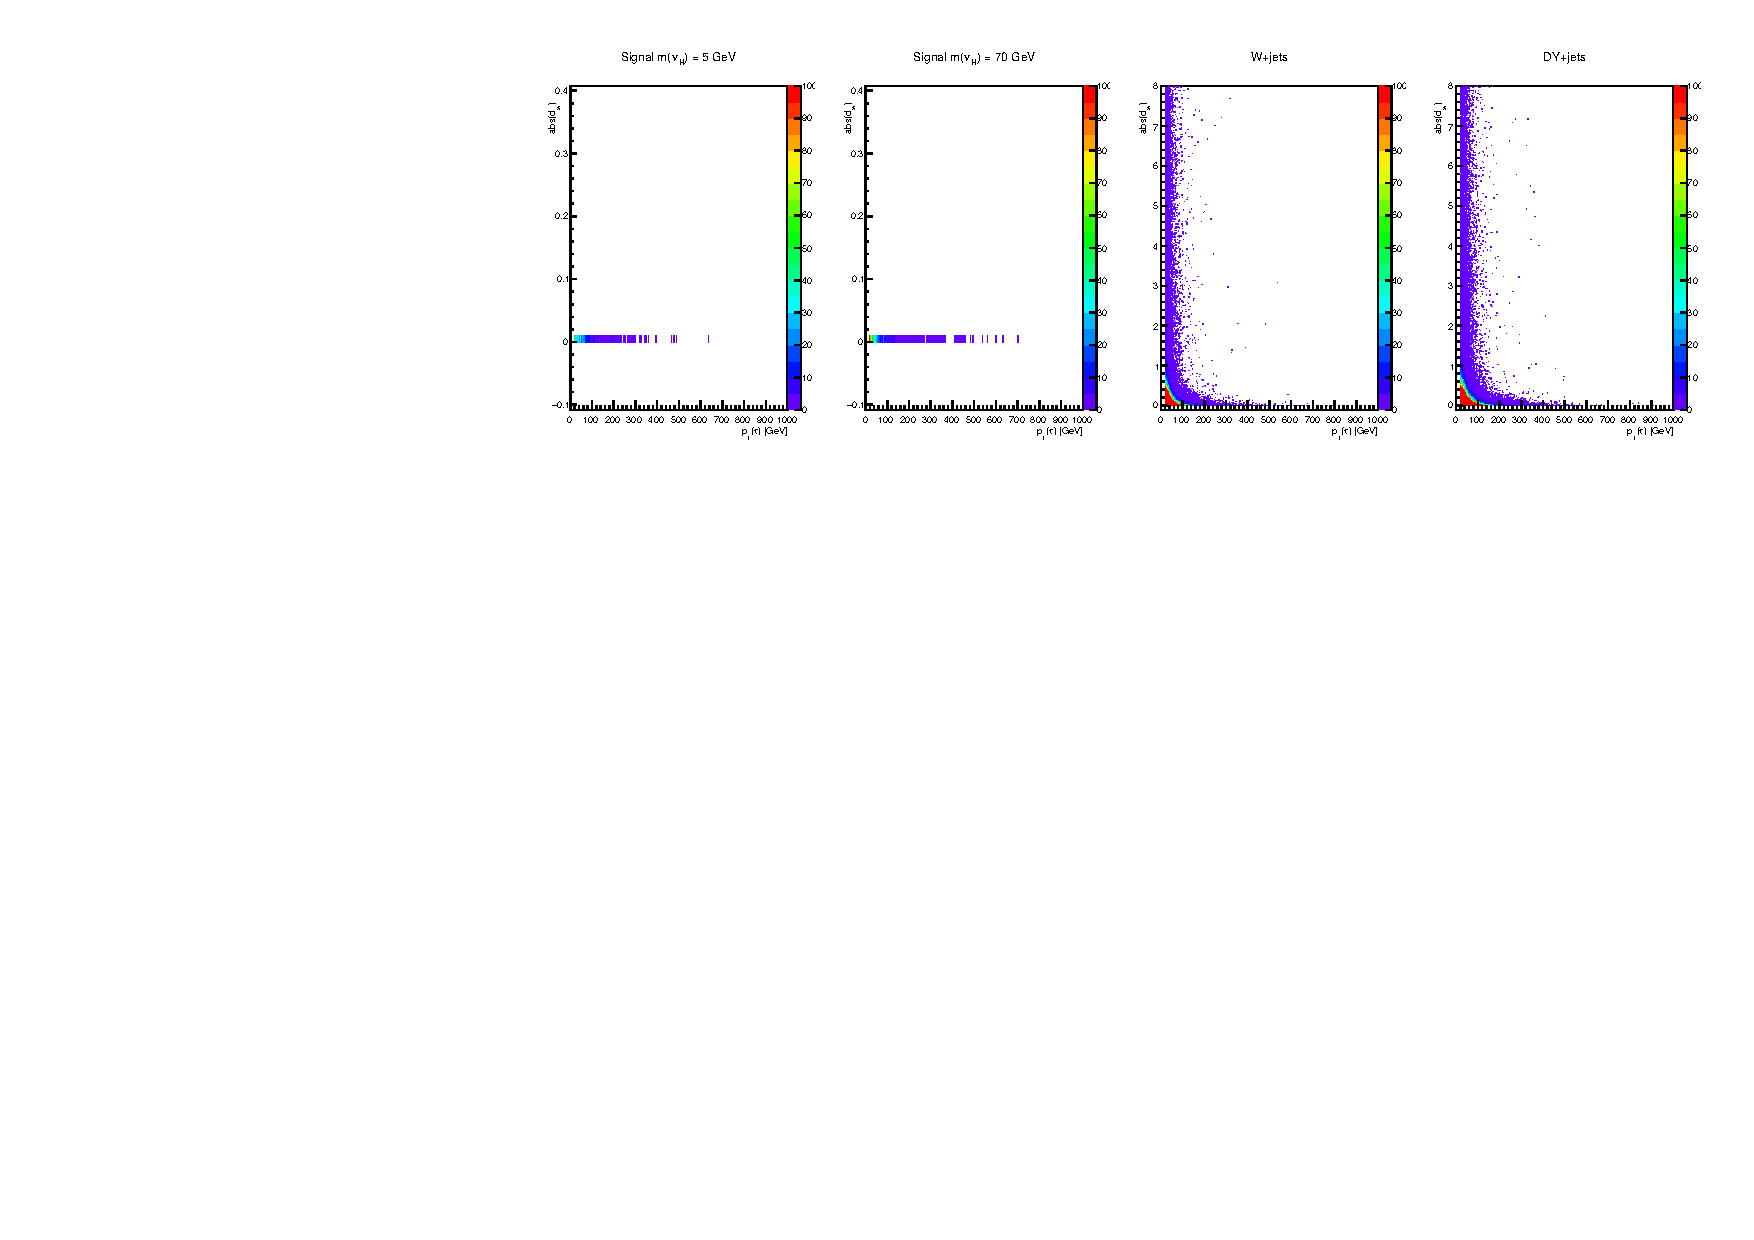
\includegraphics[width=1.15\textwidth]{./Capitulos/Analysis/ipt1_pt} 
 \label{ipt1_pt}
 \end{figure}
 
%EXPLICAR BIEN RECONSTRUCCION VERTICES Y MEJORAR GRAFICA 
 
Thus, we obtained that the signals of interest present a very low impact parameter value, while it was expected the opposite. Next, possible reasons that can explain the difference between our results and what was expected are discussed. In the first place, the quantity of signal events simulated is much smaller than the number of background events. Both simulated signals consisted of 10000 events, while the W+jets and DY+jets background samples consisted of millions of events. Thus, we had a small statistical sample and it may be necessary to generate more signal events to make the study. On the other hand, it seemed that there was a problem in the generation of the signals because their impact parameter values were only positive values. The former is not expected because there is no reason to believe that the impact parameter would have an asymmetric distribution. If this problem is solved, a cut on the impact parameter value would significantly reduce the amount of background.
